\chapter{$n$阶展开方法及其应用}\label{ch04}
在微分方程的求解中, 有许多方法都是基于齐次平衡原则发展起来的, 如\Painleve{}展开法\D 双曲正切方法和 Jacobi 椭圆函数方法等. 齐次平衡原则将方程的解设为特定函数的多项式, 通过平衡方程中两个不同最高项的阶数来确定解的阶数. 但是, 在阶数相同的两个最高项平衡时, 齐次平衡原则不能确定阶数的上界, 从而有可能产生漏解的情况. 考虑方程$u(u_t+u_{xxx})+pu_x u_{xx}=0$, 在双曲正切方法和\Painleve{}展开法中, 该方程的阶数列表为$\mbrace{2m+1,2m+3,2m+3}$, 不能基于齐次平衡原则来确定解的阶数. 本文发现, 解的阶数不仅会出现在最高$n$项的阶数中, 还会出现在最高$n$项的系数中. 因此, 本文考虑同时平衡方程中最高$n$项的阶数和系数, 提出了$n$阶展开方法. 

基于$n$阶展开方法能够补充和完善许多基于齐次平衡原则发展起来的方法. 因为非线性差分方程多项式解的求解只涉及多项式的运算, 所以本文将在\refsec{ch4sec1}中以它为例导出$n$阶展开方法. 接着, 我们将在\refsec{ch4sec2}中用图像和例子来形象地解释$n$阶展开方法的原理和作用. 随后, 本文将在\refsec{ch4sec3}中提炼出通用的$n$阶展开方法并实现一个通用的NEM软件包. 基于NEM, 本文在\refsec{ch4sec4}中实现了求非线性差分方程多项式的软件包 NLREPS. 接着, 本文在\refsec{ch4sec5}和\refsec{ch4sec6}中分别以双曲正切方法和\Painleve{}展开法为例阐述$n$阶展开方法在微分方程求解中的应用. 最后, 在\refsec{ch4sec7}中对$n$阶展开方法及其应用进行小结. 

\section{齐次平衡原则与$n$阶展开方法} \label{ch4sec1}
尽管线性差分方程的求解并没有被完全解决, 但是它的解从多项式解开始变得越来越一般. 受其发展过程的启发, 本文决定求解非线性差分方程的多项式解. 本文求解的方程形如
\begin{equation}
\sum_{k=0}^l{\mbrace{a_k(x)\prod_{i=0}^r{f^{\gamma_{ki}}(x+i)}}}=0,
\label{eq}
\end{equation}
其中 $K$是一个数域, $a_k(x)\in K[x], l>1, \gamma_{ki}\ge 0$. 在本节中, 将基于该方程多项式解的求解导出$n$阶展开方法. 

设
\begin{equation}
f(x)=\sum_{k=0}^m{\mu_kx^k},
\label{fm1}
\end{equation}
将其代入\refeqn{eq}可以求得所有次数不超过$m$的多项式解. 为了求得所有的多项式解, 我们需要找到$m$的上界.

将\refeqn{fm1}代入\refeqn{eq}后, 方程的左端仍然是一个多项式, 这个多项式的各项次数为
\begin{equation}
D = \mbrace{s_1 m+d_1,s_2 m+d_2,\cdots,s_l m+d_l},
\end{equation}
其中
\begin{equation}
\begin{aligned}
s_k&=\sum_{i=0}^r{\gamma_{ki}}, \\
d_k&=\deg a_k(x).
\end{aligned}
\label{eq-sd}
\end{equation}
$D$ 中的每一个次数都是关于 $m$ 的线性表达式, 我们称其为该项的阶数.

方程的左端为零要求整理后的多项式的各项系数为零, 从而要求最高项的系数为零. 因为各个加法项的最高项系数非零, 所以至少有两个不同的最高项进行合并才能使得整理后的多项式最高项系数为零. 从而, 有 
\begin{equation}
\left\{
\begin{array}{l}
m\in \mathbb Z_+  ,                                     \\
\exists i\neq j, s_i m+d_i=s_j m+d_j    ,               \\
\forall k \not\in \bbrace{i,j}, s_i m+d_i\ge s_k m+d_k .
\end{array}
\right.
\label{cond}
\end{equation}
上式中的三个约束条件分别被称为: 整数性约束\D 平衡性约束和最大性约束. 

(I) 如果 $s_i \neq s_j$, 则有 
\begin{equation}
m=\frac{d_j-d_i}{s_i-s_j}.
\end{equation}
如果$m$又同时满足\refeqn{cond}中的其它条件, 则称它为第一类平衡点(简称 \BPone{}). 第一类平衡点构成的集合为 
\begin{equation}
M_1=\bbrace{\left. m=\frac{d_j-d_i}{s_i-s_j}\in \mathbb Z_+\right\vert \forall k\not\in \bbrace{i,j}, s_i m+d_i\ge s_k m+d_k}.
\end{equation}

(II) 如果 $s_i = s_j, d_i=d_j$, 则能始终满足平衡性约束. 考虑最大性约束, 则有 
\begin{equation}
\left\{
\begin{aligned}
m > \frac{d_k-d_i}{s_i-s_k}, & \text{ if } s_i>s_k,  \\
m < \frac{d_k-d_i}{s_i-s_k}, & \text{ if } s_i<s_k.  \\
\end{aligned}
\right.
\end{equation}
因为\BPone{}的成立条件已经包含上述不等式中取等号的条件, 所以上述不等式不含等号. 求解上述不等式, 可以得到 
\begin{equation}
\underset{s_i>s_k}{\max}{\frac{d_k-d_i}{s_i-s_k}} < m < \underset{s_i<s_k}{\min}{\frac{d_k-d_i}{s_i-s_k}}.
\end{equation}
如果 $s_i m + d_i < \sigma m + \delta$, 则$m$存在上界. 这里, 
\begin{equation}
\begin{aligned}
\sigma &= \max ~s_k,  \\
\delta &= \underset{s_k=\sigma}{\max}{~d_k}.
\end{aligned}
\label{eq-max-sd}
\end{equation}

我们将根据$m$是否存在上界, 分两种情况进一步讨论:

(II-a) 当 $s_i m + d_i < \sigma m + \delta$时, $m$的取值范围有限. 可以得到第二类平衡点(简称 \BPtwo{}). 第二类平衡点构成的集合为
\begin{equation}
M_2=\bbrace{m\in \mathbb Z_+\left|\underset{s_i>s_k}{\max}{\frac{d_k-d_i}{s_i-s_k}} < m < \underset{s_i<s_k}{\min}{\frac{d_k-d_i}{s_i-s_k}}\right.} .
\end{equation}

(II-b) 当 $s_i m + d_i = \sigma m + \delta$ 时, 无法基于齐次平衡原则来确定$m$的上界. 因此, 我们提出了一个$n$阶展开方法来解决这个问题.

给定 $n>0$, 定义一个$m$次多项式的$n$阶展开形式为
\begin{equation}
F\sbrace{x,m,u\up n}=\sum_{k=0}^{n-1}{u_k x^{m-k}}+\OO\sbrace{x^{m-n}},
\label{npoly}
\end{equation}
其中 $u\up n=\mbrace{u_0,u_1,\cdots,u_{n-1}}$是系数向量, 而
\begin{equation}
\OO\sbrace{x^n}=\left\{
\begin{array}{cl}
\text{次数不超过}\,n\,\text{的多项式} & n\ge 0, \\
0                                    & n<0 .
\end{array}
\right.
\end{equation}

对于未知的$m$次多项式$f(x)$, 设其最高$n$项的系数为$u\up n=\mbrace{u_0,u_1,\cdots,u_{n-1}}$, 则它可以表示为 
\begin{equation}
f(x)=F\sbrace{x,m,u\up n}. \label{nepoly-f}
\end{equation}

对于一个具体的多项式
\begin{equation}
a_k(x)=\sum_{i=0}^{d_k}{a_{k,i} x^{d_k-i}}, \label{nepoly-a}
\end{equation}
设
\begin{equation}
\alpha_{k,i}=\left\{
\begin{array}{cl}
a_{k,i} & i\le \min\{n-1,d_k\}, \\
0       & i >  \min\{n-1,d_k\},
\end{array}
\right.
\end{equation}
则有
\begin{equation}
a_k(x)=F\sbrace{x,d_k,\alpha_k\up n},
\end{equation}
其中 $\alpha_k\up n=\mbrace{\alpha_{k,0},\alpha_{k,1},\cdots,\alpha_{k,n-1}}$.

于是, 在确定$n$阶展开多项式的基本运算规则之后, 就能将\refeqnn{eq}的左端改写为一个$n$阶展开多项式.

首先, 考虑移位操作
\begin{equation}
\Delta^r F\sbrace{x,m,u\up n} = F\sbrace{x+r,m,u\up n} = f(x+r).
\end{equation}
当 $r\neq 0$ 时, 有 
\begin{equation} 
\begin{aligned}
\Delta^r F\sbrace{x,m,u\up n} &= \sum_{k=0}^{n-1}{u_k (x+r)^{m-k}}+\OO\sbrace{x^{m-n}} \\
&= \sum_{k=0}^{n-1}{u_k \mbrace{\sum_{j=0}^{m-k}{\binom{m-k}{j}r^j x^{m-k-j}}}}+\OO\sbrace{x^{m-n}} \\
&= \sum_{k=0}^{n-1}{u_k \mbrace{\sum_{m-k-j>m-n}{\binom{m-k}{j}r^j x^{m-k-j}}}}+\OO\sbrace{x^{m-n}} \\
&= \sum_{k+j<n}{u_k {\binom{m-k}{j}r^j x^{m-k-j}}}+\OO\sbrace{x^{m-n}} \\
&=\sum_{p=0}^{n-1}{x^{m-p}\mbrace{\sum_{k=0}^p{u_k\binom{m-k}{p-k}r^{p-k}}}}+\OO\sbrace{x^{m-n}}\\
&=F\sbrace{x,m,v\up n}.
\end{aligned} \label{NEM-shift}
\end{equation}
其中 $v\up n=\mbrace{v_0,v_1,\cdots,v_{n-1}}$, 而
\begin{equation}
v_p=\sum_{k=0}^p{u_k\binom{m-k}{p-k}r^{p-k}}.
\end{equation}

注意到系数$v_p$是关于$m$的多项式, 所以我们不仅可以基于次数来分析$m$的取值, 还能基于系数来分析$m$的取值. 

然后, 考虑乘法 
\begin{equation}
\begin{aligned}
& F\sbrace{x,m,u \up n}\cdot F\sbrace{x,l,v\up n} \\
=& \mbrace{\sum_{k=0}^{n-1}{u_k x^{m-k}}+\OO\sbrace{x^{m-n}}}\mbrace{\sum_{k=0}^{n-1}{v_k x^{l-k}}+\OO\sbrace{x^{l-n}}} \\
=& \mbrace{\sum_{k=0}^{n-1}{u_k x^{m-k}}}\mbrace{\sum_{k=0}^{n-1}{v_k x^{l-k}}}+\OO\sbrace{x^{m+l-n}} \\
=& \sum_{p=0}^{n-1}{x^{m+l-p}\mbrace{\sum_{k=0}^p{u_k v_{p-k}}}}+\OO\sbrace{x^{m+l-n}} \\
=& F\sbrace{x,m+l,w\up n} ,
\end{aligned} \label{NEM-times}
\end{equation}
其中 $w\up n=\mbrace{w_0,w_1,\cdots,w_{n-1}}$, 而
\begin{equation}
w_p=\sum_{k=0}^p{u_k v_{p-k}}.
\end{equation}

在确定了乘法和移位操作之后, 就能将\refeqnn{eq}中的每个加法项重写为$n$阶展开多项式, 即
\begin{equation}
\begin{aligned}
a_k(x)\prod_{i=0}^r{f^{\alpha_{ki}}(x+r)}&=F\sbrace{x,d_k,\alpha_k\up n}\prod_{i=0}^r{\Delta^{\gamma_{ki}}F\sbrace{x,m,u\up n}} \\
&= F\sbrace{x,s_k m+d_k, \omega_k\up n} .
\end{aligned}
\end{equation}

最后, 考虑更为复杂的加法: 
\begin{equation}
F\sbrace{x,s_i m+d_i,u\up n}+F\sbrace{x,s_j m+d_j,v\up n}.
\end{equation}
一般情况下, 我们不能在$m$未知的情况下比较 $s_i m + d_i$ 和 $s_j m + d_j$ 大小. 但是, 假设
\begin{equation}
s_i m+d_i\ge s_j m+d_j+n, \label{cond_add}
\end{equation}
可以有 
\begin{equation}
\begin{aligned}
&F\sbrace{x,s_i m+d_i,u\up n}+F\sbrace{x,s_j m+d_j,v\up n} \\
=&\left\{
\begin{array}{cl}
    F\sbrace{x,s_i m+d_i,u\up n} & s_i>s_j,            \\
    F\sbrace{x,s_i m+d_i,w\up n} & s_i=s_j,
\end{array}
\right.
\end{aligned} \label{NEM-add}
\end{equation}
其中
\begin{equation}
w_p=\left\{
\begin{array}{cl}
u_p               & p<d_i-d_j ,   \\
u_p+v_{p-d_i+d_j} & p\ge d_i-d_j.
\end{array}
\right.
\end{equation}

最终, \refeqnn{eq} 能够被重写为
\begin{equation}
F(x,\sigma m + \delta,\Omega\up n)=0, 
\label{eq-np}
\end{equation}
其中 $\Omega\up n=\mbrace{\Omega_0,\cdots,\Omega_{n-1}}$, 而 $\Omega_k$ 则是关于 $m$ 和 $u_k$ 的多项式.

在情况(II-b)的条件下, 由\refeqn{cond_add}可知, 若要使\refeqn{eq-np}中的第$k~(k=0,1,\cdots)$个系数有效, 则需满足 
\begin{equation}
\forall s_j<\sigma, \sigma m + \delta - k > s_j m + d_j,
\end{equation}
即
\begin{equation}
m > \underline{m}_k=\underset{s_j<\sigma}{\max}{\frac{d_j-\delta+k}{\sigma-s_j}}.
\end{equation}

现在我们可以来寻找第三类平衡点(简称\BPthree{}). 因为\refeqnn{eq}的左端非零, 因此当$n$足够大时, 必然存在一个$\Omega_k\neq 0$. 设$\Omega_{k_0}$是第一个非零项. 

如果 $\Omega_{k_0}=0$ 关于 $m$ 有非负整数解 $m_0$, 则解的次数必然不超过 $m_0$. 同时, $\Omega_{k_0}$ 的有效性又要求 $m>\underline{m}_{k_0}$. 所以, 此类\BPthree{}所构成的集合为 
\begin{equation}
M_3=\bbrace{m\in \mathbb Z_+|\max\sbrace{M_1\cup M_2 \cup \bbrace{\underline{m}_{k_0}}}<m\le m_0}. \label{BP31}
\end{equation}

如果 $\Omega_{k_0}=0$ 关于 $m$ 没有非负整数解, 就意味着当 $\Omega_{k_0}$有效时(即$m>\underline{m}_{k_0}$时), 方程没有多项式解. 因此, 方程有多项式解的必要条件是 $m\le \underline{m}_{k_0}$. 从而, 此类\BPthree{}构成的集合为 
\begin{equation}
M_3=\bbrace{m\in \mathbb Z_+|\max\sbrace{M_1\cup M_2}<m\le \underline{m}_{k_0}}. \label{BP32}
\end{equation}

最终, 可以确定$m$的上界, 即
\begin{equation}
\overline m =\max\sbrace{M_1\cup M_2\cup M_3}.
\end{equation}
将 $f(x)=\sum_{k=0}^{\overline m}{\mu_k x^k}$ 代入 \refeqnn{eq}, 我们就能求得所有的多项式解.

\section{方法的可视化与典型例子}\label{ch4sec2}
基于\refeqn{cond}中的三个约束条件, 我们确定了解的次数的上界. 因为方程中每一项的次数都是关于$m$的线性表达式, 所以它们能够被看成是平面上的一条直线. 设各项次数为 
\begin{equation}
\lambda_1(m),\cdots,\lambda_l(m), \label{lines}
\end{equation}
其中 $\lambda_k(m)=s_k m+d_k$. 我们的算法等价于在折线
\begin{equation}
\lambda(m)=\max\bbrace{\lambda_1(m),\cdots,\lambda_l(m)} \label{broken_line}
\end{equation}
上寻找两条不同直线的整数交点. 

例如在\reffig{point}中, 有7条直线, 它们分别被记为$\lambda_1,\cdots,\lambda_7$. 这里, 红色表示有多条重复直线, 而黑色表示只有一条直线. 我们用虚线表示\refeqn{lines}中的直线, 用实线表示\refeqn{broken_line}中的折线. 这些直线的交点被标记为$B_1,\cdots,B_8$, 并且我们假设它们都是整点. 
\begin{figure}[htbp]
\centering
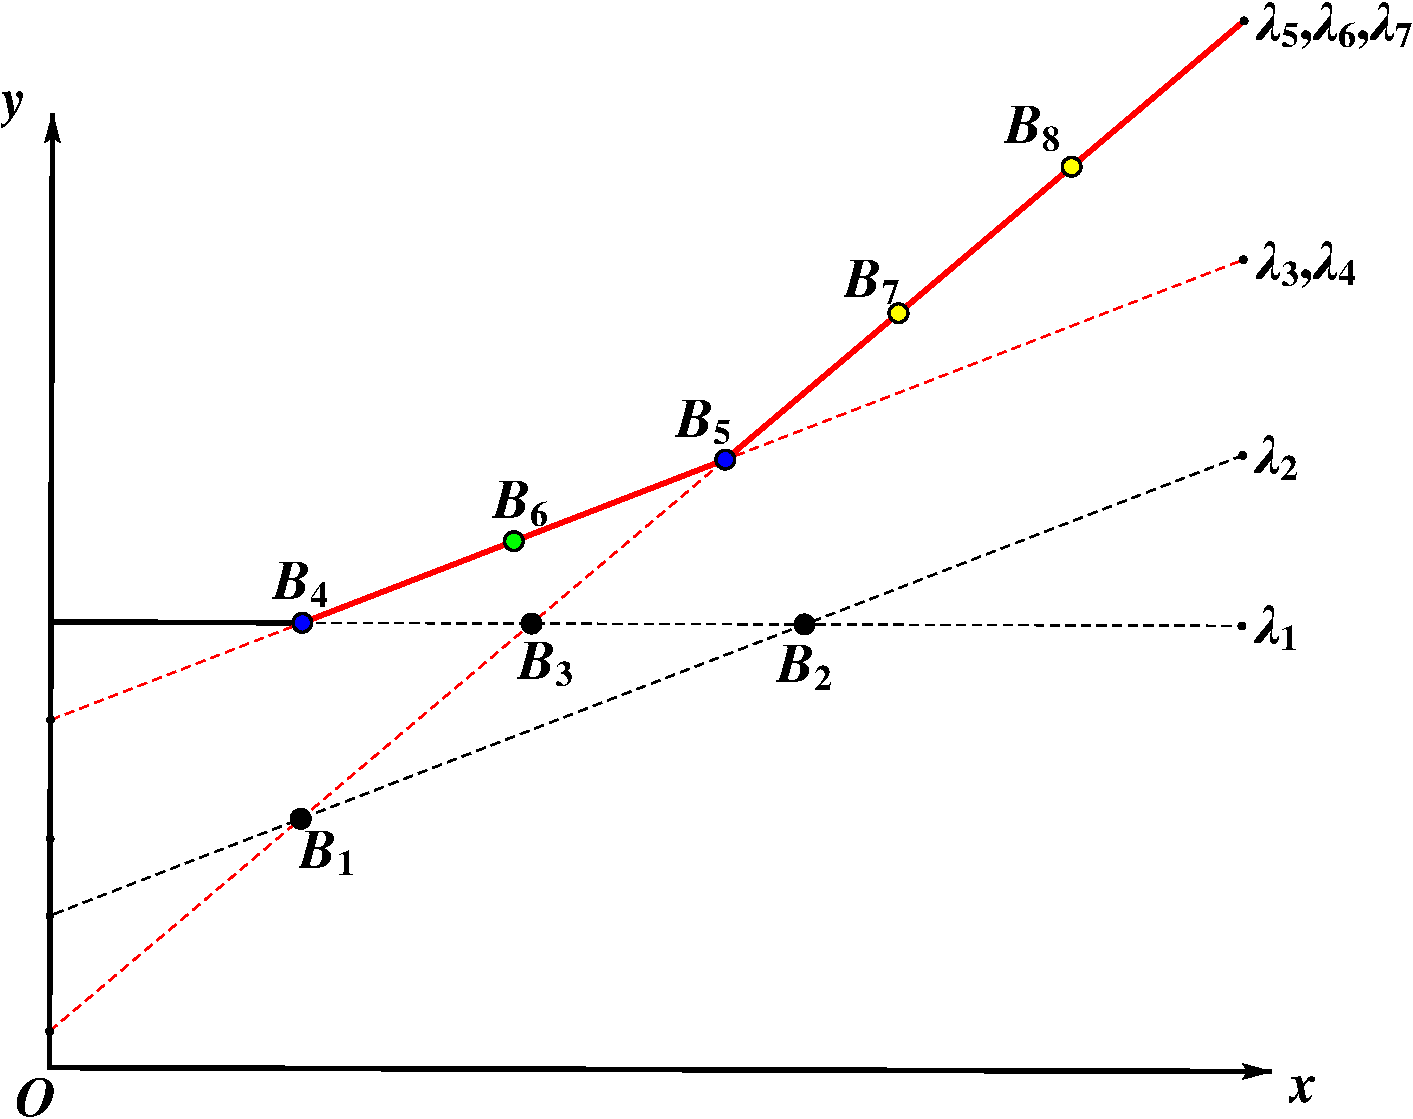
\includegraphics[width=0.6\textwidth]{fig/ps.pdf}
\caption{$n$阶展开方法的平衡点分类示意图}
\label{point}
\end{figure}
\begin{compactitem}[\textbullet]
\item 尽管$B_1,B_2,B_3$是不同直线的交点, 但是因为它们不满足最大性约束, 所以他们不是平衡点. 
\item 而$B_4,B_5$ 是不同直线的交点且满足最大性约束, 所以它们是第一类平衡点.
\item $B_6$虽然不是不同直线的交点, 但有多条直线穿过它. 又因为它在$B_4$ 和 $B_5$ 之间, 所以它是第二类平衡点.
\item 因为有多条重复直线穿过$B_7,B_8$以及它们右侧更多的整点, 且它们的右侧没有其它直线的交点, 所以它们是可能的第三类平衡点. 我们可以通过$n$阶展开方法来确定这一类平衡点的上界.
\end{compactitem}

下面将给出一些具有代表性的例子. 

\begin{example}
(\BPone{})
\begin{equation}
-x^4f(x+3)+(x+1)f(x)^2+8x^6+27x^5+28x^4+2x^3-x-1=0 \label{ep1} .
\end{equation}

该方程的阶数列表为$[m+4,2m+1,6]$. 因为没有重复的次数, 所以该方程只有\BPone{}. 基于 $m+4=6,2m+1=6$ 和 $m+4=2m+1$ 可以得出 $M_1=\{2,3\}$, 从而$\overline m = 3$. 然后, 将$f(x)=\sum\nolimits_{k=0}^3{\mu_k x^k}$ 代入原方程, 可得到如下方程组:
\begin{equation}
\left\{
\begin{array}{l}
    {\mu_{{0}}}^{2}-1=0,                                                                                                  \\
    {\mu_{{3}}}^{2}-\mu_{{3}}=0,                                                                                            \\
    {\mu_{{0}}}^{2}+2\,\mu_{{0}}\mu_{{1}}-1=0,                                                                                \\
    2\,\mu_{{0}}\mu_{{1}}+2\,\mu_{{0}}\mu_{{2}}+{\mu_{{1}}}^{2}=0,                                                                \\
    2\,\mu_{{2}}\mu_{{3}}+{\mu_{{3}}}^{2}-\mu_{{2}}-9\,\mu_{{3}}+8=0,                                                             \\
    2\,\mu_{{0}}\mu_{{2}}+2\,\mu_{{0}}\mu_{{3}}+{\mu_{{1}}}^{2}+2\,\mu_{{1}}\mu_{{2}}+2=0,                                            \\
    2\,\mu_{{1}}\mu_{{3}}+{\mu_{{2}}}^{2}+2\,\mu_{{2}}\mu_{{3}}-\mu_{{1}}-6\,\mu_{{2}}-27\,\mu_{{3}}+27=0,                              \\
    2\,\mu_{{0}}\mu_{{3}}+2\,\mu_{{1}}\mu_{{2}}+2\,\mu_{{1}}\mu_{{3}}+{\mu_{{2}}}^{2}-\mu_{{0}}-3\,\mu_{{1}}-9\,\mu_{{2}}-27\,\mu_{{3}}+28=0.
\end{array}
\right.
\label{ceqs}
\end{equation}
可以求出\refeqnn{ceqs}的解为$\{\mu_0=-1,\mu_1=0,\mu_2=0,\mu_3=1\}$. 最终, \refeqnn{ep1}的多项式解为$f(x)=x^3-1$.
\end{example}

\begin{example}
(\BPtwo{})
\begin{equation}
x^2f(x)f(x+1)f(x+2)+(1-x^9)f(x)+(x^4-x^9)f(x+1)+2x^9f(x+2)-\sum_{k=0}^{10}{c_k x^k}=0, \label{ep2}
\end{equation}
其中$[c_0,\cdots,c_{10}]=[1,1,22,57,85,72,35,9,1,10,6]$. 该方程的阶数列表为$[3m+2,m+9,m+9,m+9,10]$. 从$m+9=10$可以得到第一类平衡点$M_1=\{1\}$. 因为$m+9$有多个, 且它关于$m$的系数不是最大的, 所以该方程有\BPtwo{}. 从$\{m+9> 10,m+9> 3m+2\}$可以得出$m< 7/2$. 因此, $\overline m=3$. 然后, 可以解得原方程的多项式解为$f(x)=x^2+x+1$. 显然, 如果不考虑\BPtwo{}, 我们将无法求出该方程的多项式解. 
\end{example}

\begin{example} \label{examp-3}
(\BPthree{}, 2阶展开)
\begin{equation}
(x+2)f(x)-(x-1)f(x+1)=0. \label{ep3}
\end{equation}
因为该方程的阶数列表为$[m+1,m+1]$, 所以它只有\BPthree{}. 基于2阶展开, 即将$f(x)=u_0 x^m + u_1 x^{m-1} + \OO(x^{m-2})$ 代入到原方程中, 可以得到
\begin{equation}
(-u_0 m+3u_0)x^m+\OO(x^{m-1})=0.
\end{equation}
从 $-u_0 m+3u_0=0$ 可以解得 $m=3$. 然后, 可以解得该方程的多项式解 $f(x)=c(x^3-x)$, 其中 $c$ 是任意常数.
\end{example}

\begin{example}
(\BPthree{}, 高阶展开)
\begin{equation}
-2x^5f(x)f(x+2)+x^4f(x)^2+(2x^5-x^4)f(x+1)^2-\sum_{k=0}^{22}{c_k x^k}=0, \label{ep4}
\end{equation}
其中 $[c_0,\cdots,c_{22}]=$[0, 0, 0, 0, 1, 2046, 10140, 22340, 28095, 20730, 7788, 6120, 30600, 84180, 151164, 199504, 199710, 151380, 85560, 35136, 10035, 1830, 170]. 该方程的阶数列表为 $[2m+5,2m+4,2m+5,22]$. 由 $2m+5=22$ 可得 $ m=17/2$, 该方程没有\BPone{}. 所以该方程只有\BPthree{}. 在该方程的$n$阶展开中, 第一个非零项为 
\begin{equation}
\Omega_3 = 2m^2u_0^2-3mu_0^2-2u_0u_1.
\end{equation}
因为$\Omega_3=0$关于$m$没有正整数解, 所以当$\Omega_3$有效时, 方程没有多项式解. 换句话说, 只有$2m+5>22+3$不成立, 即$m\le 10$时, 才有多项式解. 从而, $\overline m =10$, 可以得到\refeqnn{ep4} 的多项式解为 $f(x)=\pm (x^{10}-1)$.
\end{example}

\begin{example}
(应用, 2阶展开)

为了计算 
\begin{equation}
    S(x)=\sum_{k=0}^x{k^{10}}
\end{equation}
的闭形式解, 可以构造差分方程
\begin{equation}
    S(x)-S(x-1)=x^{10}, S(0)=0. \label{seq}
\end{equation}
该方程的阶数列表为$\mbrace{m,m,10}$. 此时, $m=10$ 是 \BPone{}. 因为这里有两个重复的$m$, 所以需要考虑\BPthree{}. 该方程的二阶展开为
\begin{equation}
u_0m x^{m-1}+\OO(x^{m-2})=0.   
\end{equation}
因为当$m-1>10$时, $\Omega_1=u_0m$有效, 方程没有多项式解. 所以, 必须有$m\le 11$. 从而, $\overline m=11$, 可以得到原方程的多项式解为
\begin{equation}
S(x)=\frac{5}{66}x-\frac{1}{2}x^3+x^5-x^7+\frac{5}{6}x^9+\frac{1}{2}x^{10}+\frac{1}{11}x^{11}.
\end{equation}
对这个例子, 如果不考虑第三类平衡点, 我们将不能获得其多项式解. 

另一方面, \refeqnn{seq}是一个线性方程, 也可以采用其它方法\cite{Abramov1989polynomial,Abramov1995polynomial}求其多项式解. 但是, 这个方程在我们的方法中是通过2阶展开求解的, 这也说明了$n$阶展开的必要性. 
\end{example}

\begin{example}
(应用, logistic方程, 也称虫口方程)

因为我们的算法可以求出所有的多项式解, 所以如果基于我们的算法没有获得多项式解则表示方程没有多项式解. 考虑著名的logistic 方程\cite{may1976simple}
\begin{equation}
    f(x+1)=r f(x)\sbrace{1-f(x)},
\end{equation}
其中 $r$ 是一个常数. 该方程的阶数列表为 $\mbrace{2m,m,m}$. 因为 $2m\ge m$, 所以该方程只有\BPone{}, 即$2m=m\Rightarrow m=0$. 可以的得出, 该方程除了$f(x)=0$和$f(x)=(r-1)/r$以外, 没有其它非平凡的多项式解.
\end{example}

\begin{example}
(应用, Riccati方程)

对于 Riccati 方程\cite{bittanti2012riccati}
\begin{equation}
    f(x+1)f(x)+A(x)f(x)+B(x)f(x+1)=C(x), \label{raeq}
\end{equation} 
其中$A(x),B(x)$ 和 $C(x)$ 是多项式系数, 我们取 
\begin{equation}
\begin{aligned}
A(x)&= -\frac{1}{2}\sbrace{x^5+5x^4-40x^2-2}, \\ 
B(x)&= -\frac{1}{2}\sbrace{x^5+10x^3-x-2}, \\ 
C(x)&= -x\sbrace{x+1}\sbrace{48x^4+20x^2-5x-3}.
\end{aligned}
\end{equation}
该方程的阶数列表为$\mbrace{2m,m+5,m+5,6}$. 对于该方程的平衡点的分类讨论如\reftab{tb}所示.

\begin{table}[htbp]
\centering
\caption{关于 Riccati 方程的平衡点的分类讨论}\label{tb}
\begin{tabular}{ccc}
\hline
平衡点类型 & 平衡方程 & 平衡点  \\ 
\hline
\BPone{}  & $2m=m+5\ge 6$            & $m=5$             \\ 
\BPone{}  & $2m=6\ge m+5$            & $m\in \varnothing$             \\ 
\BPone{}  & $m+5=6\ge 2m$            & $m=1$             \\ 
\BPtwo{}  & $m+5>\max\bbrace{2m,6}$  & $m\in \bbrace{2,3,4}$ \\
\hline
\end{tabular}
\end{table}
从\reftab{tb}中可以得出: $M_1=\bbrace{1,5},M_2=\bbrace{2,3,4}$. 因此, $\overline m=5$. 最终, 可以得到该方程的多项式解 $f(x)=x^5-x$. 

在 Maple 中, 使用 \cd{rsolve} 求解\refeqnn{raeq}会得到
\begin{equation}
\begin{aligned}
    f(x)&=(f \left( 0 \right) \alpha(x)\,{x}^{5}+f \left( 0 \right) \beta(x)\,{x}^{5}+10\,f \left( 0 \right) \alpha(x)\,{x}^{3}\\
    &-10\,f \left( 0 \right) \beta(x)\,{x}^{3}+2\,{x}^{5}-f \left( 0 \right) \alpha(x)\,x-f \left( 0 \right) \beta(x)\,x\\
    &-2\,f \left( 0 \right) \alpha(x)+2\,f \left( 0 \right) \beta(x)-2\,x)/(2+2f(0)\alpha(x)) ,
\end{aligned} \label{rasol_real}
\end{equation}
其中
\begin{equation}
\begin{aligned}
&\alpha(x)=\sum_{k_1=0}^{x-1}\mbrace{
    \frac{(-1)^{k_1}p(k_1)}{q(k_1)}\prod_{k_0=0}^{k_1}{
        \frac{q(k_0)}{p(k_0)}
    }
}, \\
&\beta(x)=\sum_{k_1=0}^{x}\mbrace{
    \frac{(-1)^{k_1}p(k_1)}{q(k_1)}\prod_{k_0=0}^{k_1}{
        \frac{q(k_0)}{p(k_0)}
    }
}, \\
&p(x)=x^5+5x^4-20x^2-26x+8, \\
&q(x)=x^5+5x^4+20x^3+10x^2+8x+2. 
\end{aligned}
\end{equation}
将 $f(0)=0$ 代入\refeqn{rasol_real}, 可以得到 $f(x)=x^5-x$. 这表示该多项式解是在初始条件 $f(0)=0$ 下的解. 此外, 需要注意的是, 使用 \cd{LRETools[riccati]} 来求解\refeqnn{raeq}将得到错误的解, 这显然是该函数的一个BUG. 
\end{example}

\section{NEM软件包的实现}\label{ch4sec3}
在上文中, 我们以差分方程多项式解的求解为例, 阐述了$n$阶展开方法的思路和步骤. 实际上, $n$阶展开方法也能用于完善其它基于齐次平衡原则发展起来的方法. 为了能够更方便地将$n$阶展开方法应用到相关问题中, 本文决定将$n$阶展开方法单独实现为 NEM 软件包.

从上文的分析可以看出, 在计算\BPone{}和\BPtwo{}时, 只需要关注方程的各项次数, 而计算\BPthree{}则需要借助于$n$阶展开多项式来计算最高$n$的系数. 事实上, 只要列出了$n$阶展开多项式, 也能获得方程各项的次数. 因此, 我们将$n$阶展开多项式作为NEM的输入对象. 在应用到具体问题时, 只需将对应问题中的各项转化为$n$阶展开多项式, 就能调用NEM来确定平衡点的上界, 后续的求解则交给对应问题的相关程序进行解决. 

在NEM软件包中, 我们将$n$阶展开多项式实现为\cd{NEPoly}对象. \cd{NEPoly}对象有三个关键属性: $p,q$和$u$. 其中 $pm+q$就是该多项式的次数, 而$u$则是最高$n$项的系数. 并且, \cd{NEPoly}对象还根据\refeqn{NEM-shift}\D \refeqn{NEM-times} 和 \refeqn{NEM-add} 分别实现了移位\D 乘法和加法操作. 此外, 为了能够将程序应用到微分方程求解的相关问题中, 我们还推导了微分的计算规则:
\begin{equation}
\begin{aligned}
& \DIF{t}F\sbrace{x,m,u\up{n}}  \\
=& \DIF{t}\sbrace{\sum_{k=0}^{n-1}{u_k x^{m-k}}+\OO(x^{m-n})} \\
=& \sum_{k=0}^{n-1}{\DIFF{u_k}{t}x^{m-k}}+\DIFF{x}{t}\cdot\sum_{k=0}^{n-1}{u_k (m-k) x^{m-k-1}}+\DIFF{x}{t}\cdot\OO(x^{m-n-1}) \\
=& \sum_{k=0}^{n-1}{\DIFF{u_k}{t}x^{m-k}}+\DIFF{x}{t}\cdot\sbrace{\sum_{k=0}^{n-1}{u_k (m-k) x^{(m-1)-k}}+\OO\sbrace{x^{(m-1)-n)}}} \\ 
=& F\sbrace{x,m,v\up{n}}+\DIFF{x}{t}\cdot F\sbrace{x,m-1,w\up{n}}, 
\end{aligned}\label{NEM-diff}
\end{equation}
其中 
\begin{equation}
v_p=\DIFF{u_p}{t}, w_p=u_p(m-p).
\end{equation}
只需将$\DIFF{x}{t}$也表示成关于$x$的$n$阶展开多项式, 就能使得\cd{NEPoly}关于导数的计算结果也是$n$阶展开多项式. 

在实现了\cd{NEPoly}之后, 我们实现了NEM的核心接口\cd{nem(vs)}, 其输入参数\cd{vs}是一个\cd{NEPoly}列表, 表示方程中各个加法项转化为$n$阶展开多项式的结果. \cd{nem(vs)}的核心逻辑如\refalg{nem}所示. 

\begin{algorithm}[H]
\newcommand{\kw}[1]{\mathbf{~#1~}}
\newcommand{\Fcn}[1]{\mathtt{#1}}
\renewcommand{\lfrac}[2]{\sbrace{#1}/\sbrace{#2}}
\caption{$n$阶展开方法的核心算法 \cd{nem(vs)}}\label{nem}
\KwIn{\cd{NEPoly}对象的列表.}
\KwOut{平衡点上界, $-\infty$ 表示没有找到平衡点.}
$s,d,\sigma,\delta,l\gets \Fcn{getOrders}(vs)$\tcp*[r]{从输入对象中获取相关次数}
$m_1,m_2,m_3\gets -\infty$\tcp*[r]{初始化三种类型平衡点的上界.}
$needBP3\gets\kw{false}$\tcp*[r]{用于记录是否需要 \BPthree{}.}
\For{$i \kw{from} 1 \kw{to} l$}{\label{for-1-start}
    \For{$j \kw{from} i+1 \kw{to} l$}{
        \uIf(\tcp*[f]{寻找 \BPone{}.}){$s_i\neq s_j$}{
            $m\gets (d_j-d_i)/(s_i-s_j)$\;
            \If{$m\in \mathbb Z_+ \kw{and} s_im+d_i\ge \max\{s_km+d_k\}$}{
                $m_1\gets \max(m,m_1)$\;
            }
        }\ElseIf(\tcp*[f]{寻找 \BPtwo{}.}){$s_i=s_j \kw{and} d_i=d_j$}{
            \If(\tcp*[f]{判定是否需要\BPthree{}.}){$s_i=\sigma \kw{and} d_i=\delta$}{
                $needBP3\gets \kw{true}$;~\textbf{continue}\;
            }
            $lb\gets \floor{\underset{s_i>s_k}{\max}{\lfrac{d_k-d_i}{s_i-s_k}}}+1$\;
            $ub\gets \ceil{\underset{s_i<s_k}{\min}{\lfrac{d_k-d_i}{s_i-s_k}}}-1$\;
            \If{$ub\neq +\infty \kw{and} lb\le ub \kw{and} ub\ge 0$}{
                $m_2\gets \max(ub,m_2)$\;
            }
        }
    }
}\label{for-1-end}
\If(\tcp*[f]{寻找 \BPthree{}.}){$needBP3$}{
    $r\gets \sum_{v\in vs}{v}$;~$\Omega\gets r.u$\; \label{add-nem}
    \For{$k \kw{from} 0 \kw{to} n-1$}{\label{for-2-start}
        \If{$\Omega_k\neq 0$}{
            $sol\gets \Fcn{solve}(\Omega_k=0,m)$\;
            $m_{31}\gets \max(sol \bigcap \mathbb{Z}_+)$\tcp*[r]{有解时的上界}
            $m_{32}\gets \floor{\underset{s_j<\sigma}{\max}{\lfrac{d_j-\delta+k}{\sigma-s_j}}}$\tcp*[r]{无解时的上界}
            $m_3\gets \max(m_{31},m_{32})$\;
            \textbf{break}\;
        }
    }\label{for-2-end}
    \If{$m_3=-\infty$}{
        \cd{warning}(`$n$ need be increased.')\;
    }
}
\Return{$\overline m= \max(m_1,m_2,m_3)$}\;
\end{algorithm}

在\refalg{nem}中, 首先按照前文的定义, 从\cd{NEPoly}对象中提取相关次数. 然后, 在\refcln{for-1-start}到\refcln{for-1-end}中, 基于这些次数寻找\BPone{}和\BPtwo{}. 在此过程中, 我们也会检测当前问题是否需要继续寻找\BPthree{}. 在这个过程中, 需要对$l$个输入项进行两两比较, 在内部的计算中也需要寻找这$l$个对象中的相关最值, 所以, 这个过程的时间复杂度为$\OC(l^3)$.

若需要继续计算\BPthree{}, 我们将在\refcln{add-nem}中对输入的\cd{NEPoly}对象求和, 然后在\ref{for-2-start}-\ref{for-2-end}行中寻找\BPthree{}. 这里, $m_{31}$是$\Omega_{k_0}=0$关于$m$有解时\BPthree{}的上界, 而$m_{32}$则是无解时的上界. 因为这两者在其中一个非负时, 另一个必然为$-\infty$, 所以可以取两者的最大值来确定\BPthree{}的上界. 事实上, $m_{31}$和$m_{32}$分别对应了\refeqn{BP31}和\refeqn{BP32}的上界. 此外, 如果在当前$n$项中并未找到非零系数, 则程序会提醒用户增大展开阶数继续尝试. 在这一部分, 程序首先对$l$个输入项求和, 这部分时间复杂度为$\OC(nl)$. 然后, 程序要在$n$个展开系数中寻找非零项, 找到之后需要计算$l$个输入项的最值, 不考虑求解方程的复杂度, 则其时间复杂度为$\OC(n+l)$.

最后, 取三类平衡点的最大值就能确定平衡点的上界. 最终, \refalg{nem}的时间复杂度为$\OC(l^3+nl+n+l)$. 当$n$没有远大于$l$时, \refalg{nem}的时间复杂度等价于$\OC(l^3)$.

\section{NLREPS 软件包的实现与测试}\label{ch4sec4}

基于NEM, 我们实现了求解非线性差分方程多项式解的软件包NLREPS.
\begin{compactenum}[(1)]
\item 首先, 对于形如\refeqn{eq}的输入方程, 将各项系数$a_k(x)$用\refeqn{nepoly-a}转化为\cd{NEPoly}对象, 将未知函数$f(x)$按照\refeqn{nepoly-f}转化为\cd{NEPoly}对象. 
\item 然后, 调用\cd{NEPoly}的内置功能, 基于\refeqn{NEM-shift}计算移位, 基于\refeqn{NEM-times}计算乘法, 得到各个加法项对应的\cd{NEPoly}对象. 
\item 接着, 通过调用\refalg{nem}中的\cd{nem}函数, 计算平衡点的上界$\overline{m}$.
\item 最后, 用待定系数法, 将$f(x)=\sum_{k=0}^{\overline{m}}{\mu_k x^k}$代入原方程求解即可. 
\end{compactenum}

按照上述方法, 我们实现了NLREPS, 其核心接口为
\begin{verbatim}
nlreps(eq,fx,{nExpand,inits});
\end{verbatim}
其中
\begin{compactitem}[\textbullet]
\item \cd{eq} 表示输入的方程.
\item \cd{fx} 表示需要求解的未知函数, 如$f(x)$.
\item \cd{nExpand} 表示展开阶数. 这个参数是可选的, 默认值为\cd{nExpand=5}. 
\item \cd{inits} 表示初始条件, 例如 \cd{\{f(0)=0, f(1)=1\}}. 这个参数也是可选的, 默认为空集, 表示没有初始条件. 
\end{compactitem}

例如, 对于例\ref{examp-3}中的问题, 若添加初始条件$\{f(0)=-1\}$, 并指定展开阶数为4, 则调用方式为
\begin{verbatim}
nlreps(eq,f(x),nExpand=4,inits={f(0)=-1});
\end{verbatim}
然后, 就能得到解 $\{f(x)=x^{10}-1\}$.

为了测试NLREPS的求解性能, 我们随机生成了1000个不同规模的问题进行测试. 我们产生测试用例的方法如下: 将 
\begin{equation}
    F=\sum_{k=0}^l{\mbrace{a_k(x)\prod_{i=0}^r{f^{\gamma_{ki}}(x+i)}}}
\end{equation}
看作是关于$f(x),\cdots,f(x+r)$的多元多项式, 其系数为 $a_k(x)$. 对于这个多项式, 取
\begin{equation}
\begin{aligned}
&\max{\rm deg}(a_k(x))=\max d_k=10,\\ 
&\max{\rm deg}(F)=\max s_k=5, \\
&l\in [2,400], r=5.
\end{aligned}
\end{equation}
生成$F$之后, 我们生成一个随机的解$f^*(x)$代入$F$得到$g(x)$, 最终得到方程$F-g(x)=0$. 其中 ${\rm deg}(f^*(x))\le 10$. 生成1000个测试用例之后, 我们从3个方面对它们进行分析. 

首先, 我们考虑测试\cd{nlreps}的运行时间. 因为求解代数方程组并不是NLREPS的主要职责, 所以只计算\cd{nem}的运行时间. 我们取展开阶数为5进行测试, 所得结果如\reffig{t-nem}所示. 从\reffig{t-nem}中可以看出, 运行时间关于输入规模的增长是多项式的, 这符合前文中的理论分析. 
\begin{figure}[htbp]
\centering
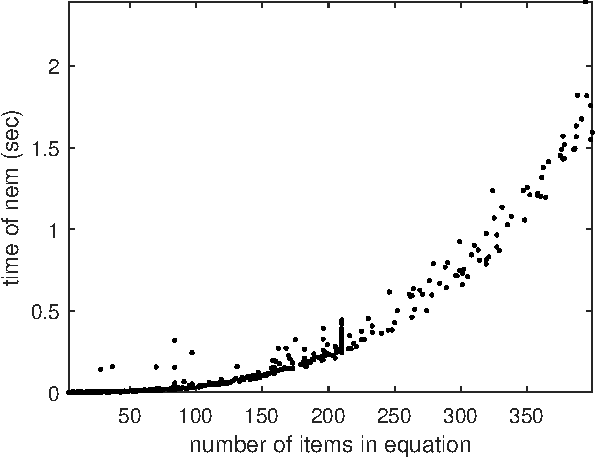
\includegraphics[width=.5\textwidth]{fig/t-nem.pdf}
\caption{NEM 的时间复杂度}
\label{t-nem}
\end{figure}

然后, 我们来关注平衡点类型的分布. 因为一共有三种平衡点, 所以我们用一个长度为3的二进制序列来表示一个方程的平衡点类型. 例如\cd{100}表示只有\BPone{}. 从\reffig{d-bps}可以看出, 几乎每个方程都有\BPone{}, 大部分方程在具有\BPone{}的同时还具有\BPthree{}. 在我们的测试中, 有2个方程只有\BPthree{}, 没有一个方程有\BPtwo{}. 这说明对于大部分的方程, 齐次平衡原则虽然能够直接求解, 但是不能排除漏解的可能性.


最后, 我们来关注一下方程的最小展开阶数. 方程的最小展开阶数指的是方程在展开后第一个非零系数出现的位置. 从\reffig{d-nExpand}中可以看出, 在我们的测试中, 只有2个例子需要二阶展开. 事实上, 这两个方程恰好是那两个只有\BPthree{}的方程. 这说明较小的展开阶数就能解决大部分的问题. 

\begin{figure}[htbp]
\centering
\subfigure[平衡点类型分布 \label{d-bps}]{
    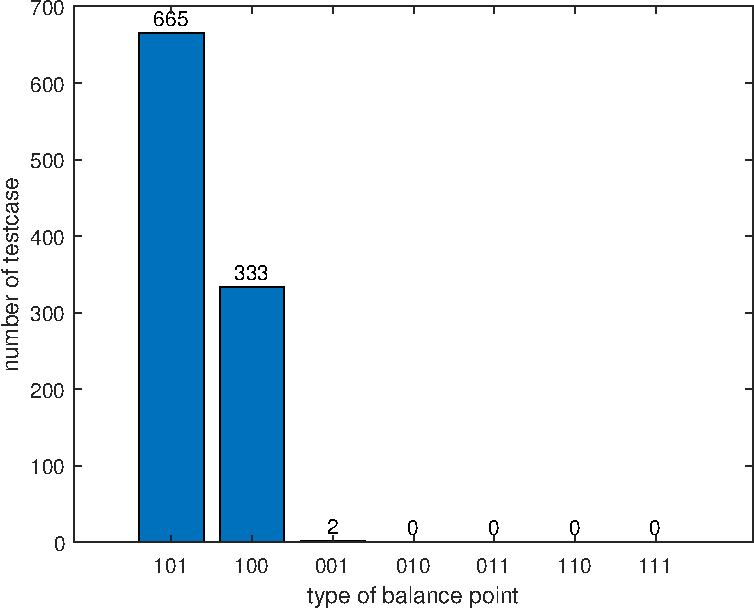
\includegraphics[width=0.45\textwidth]{fig/d-bpType.pdf}
}
\subfigure[最小展开阶数分布 \label{d-nExpand}]{
    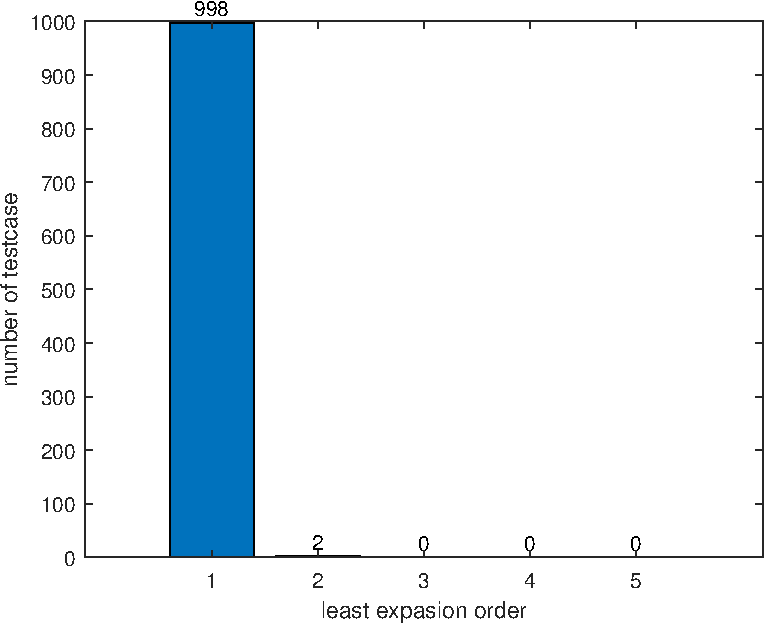
\includegraphics[width=0.45\textwidth]{fig/d-nExpand.pdf}
}
\caption{平衡点类型与最小展开阶数的分布图}
\end{figure}

\section{$n$阶展开方法在双曲正切方法中的应用}\label{ch4sec5}
和\refchp{ch02}一样, 双曲正切方法的求解对象也是非线性演化方程
\begin{equation}
    U\sbrace{u,u\up{1},u\up{2},\cdots}=0,
\end{equation}
其中 $u=u(x_1,\cdots,x_n)$, 而$U$则是关于$u$及其导数的多项式. 

在双曲正切方法中, 首先引入行波变换 
\begin{equation}
    \xi = p_1 x_1 +\cdots + p_n x_n + p_{n+1}.  \label{tanh-tw}
\end{equation}
根据链式求导法则可得
\begin{equation}
    \DIFF{u}{x_k}=\DIFF{u}{\xi}\DIFF{\xi}{x_k}=p_k\DIFF{u}{\xi}.
\end{equation}
基于上述行波变换, 可将原方程转化为关于$u(\xi)$的常微分方程
\begin{equation}
    V(u,u',u'',\cdots)=0. \label{odeq}
\end{equation}

接着, 假设\refeqnn{odeq}存在如下形式的解:
\begin{equation}
    u(\xi)=\sum_{k=0}^m{a_k \tanh^k(\xi)}. \label{tanh-poly}
\end{equation}
在原本的双曲正切方法中, 基于齐次平衡原则来确定$m$的上界. 现在, 我们可以基于$n$阶展开方法来完善它. 

和前文一样, 我们用$F(x,m,\mu\up{n})$来表示关于$x$的$m$次$n$阶展开多项式, 其最高$n$项的系数为$\mu\up{n}$. 于是, 可以将$u(\xi)$设为
\begin{equation}
    u(\xi)=F\sbrace{\tanh(\xi),m,\alpha\up{n}}.
\end{equation}

由\refeqn{NEM-diff}可知, 要使$u$关于$\xi$的导数也能表示为$n$阶展开多项式, 只需将$\DIF{\xi}\tanh(\xi)$表示为$n$阶展开多项式即可. 我们有 
\begin{equation}
    \DIFF{\tanh(\xi)}{\xi}=1-\tanh^2(\xi)=F\sbrace{\tanh(\xi),2,[-1,0,1]}.
\end{equation}
事实上, \cd{NEPoly}对象已经自动实现了上述转换. 将$u(\xi)$转化为\cd{NEPoly}对象之后, 代入\refeqnn{odeq}, 基于\cd{NEPoly}的微分和乘法操作将\refeqnn{odeq}的所有加法项转化为\cd{NEPoly}列表, 就能调用\cd{nem}求得平衡点的上界$\overline{m}$.

最后, 将$u(\xi)=\sum_{k=0}^{\overline{m}}{a_k \tanh^k(\xi)}$代入\refeqnn{odeq}就能求得原方程的双曲正切函数解.  此外, 我们在输出时还删除了平凡的解. 按照\refchp{ch03}的做法, 我们也对非平凡的双曲函数解定义了避免取值集合
\begin{equation}
    S=\bbrace{\bbrace{p_k=0}|1\le k \le n} \cup \bbrace{a_1=0,\cdots,a_m=0}.
\end{equation}
式中第一个集合保证解的维数不会退化, 第二个集合保证解不是常数. 

基于上述过程, 我们实现了 NCTM 软件包. NCTM 的核心接口为
\begin{verbatim}
sh:=nctm(eq,a,p,{SP,nExpand});
\end{verbatim}
其中
\begin{compactitem}[\textbullet]
\item \cd{eq} 表示输入的方程.
\item \cd{a} 表示\refeqn{tanh-poly}中的待定系数的变量名.
\item \cd{p} 可以是一个变量名, 也可是一个变量名列表, 用于指定\refeqn{tanh-tw}中行波变换的系数.
\item 可选参数\cd{SP}表示方程中可以求解的参数. 因为对于一些带参方程, 有时需要探索方程是否在某些参数条件下有解.
\item 可选参数\cd{nExpand}表示$n$阶展开的阶数, 默认值为2.
\item 返回结果\cd{sh}是一个\cd{SolHolder}对象, 它和TwSolver中的\cd{SolHolder}对象一样, 提供了获取解的表达式\D 验证解和绘制解等功能. 
\end{compactitem}

接下来, 我们用几个典型的例子来展示 NCTM 的基本用法, 以及它相对于现有双曲正切函数法的软件包的改进. 在\refchp{ch01}中, 我们介绍了许多关于双曲正切方法的机械化工作. 其中 从 Maple 9.5 开始引入的 \cd{PDEtools:-TWSolutions} 函数兼容性好, 能够求解高维的方程, 所以我们主要以它为例进行比较. 

\begin{example}(1+1)维 Fisher 方程, 用于展示基本用法.

考虑(1+1)维 Fisher 方程\cite{guo1991analytic},
\begin{equation}
    u_t-u_{x,x}-u(1-u)=0.
\end{equation}
取行波变换$\xi=kx+ct+\eta$, 则调用语句为
\begin{verbatim}
sh:=nctm(eq,a,[k,c,eta]);
\end{verbatim}
最终, NCTM确定$m=2$, 从而确定解的假设形式为 
\begin{eqnarray}
    u(\xi)=a_0+a_1 \tanh(\xi)+a_2\tanh^2(\xi).
\end{eqnarray}
通过求解相应的非线性代数方程组, \cd{NTCM}推导出4个解. 调用 
\begin{verbatim}
sols:=sh:-get_sols()
\end{verbatim}
可以返回 4 组参数关系
\begin{equation}
    \bbrace{a_0=a_2=\frac{1}{4},a_1=\pm \frac{1}{2},k=\pm \frac{\sqrt 6}{12},c=\frac{5}{6}a_1}. \label{para-rel}
\end{equation}
这4组解和\cd{PDEtools:-TWSolutions}给出的解是等价的.

如果想要获取解的表达式, 则可以调用\cd{sh:-get\_sol}. 在这个例子中, 调用
\begin{verbatim}
sh:-get_sol(sols[4]);
\end{verbatim}
可以得到
\begin{equation}
    u(x,t)=\frac{1}{4}\sbrace{1+2\tanh\sbrace{\frac{1}{12}(\sqrt{6}x+5t)+\eta}+\tanh^2\sbrace{\frac{1}{12}(\sqrt{6}x+5t)+\eta}}. \label{fisher-sol-4}
\end{equation}

如果用户想验证所得的解是否满足原方程, 则可以调用
\begin{verbatim}
sh:-verify_sol(sol);
\end{verbatim}
其中\cd{sol}是一个参数关系的集合.

最后, 用户还能对所得的解进行作图. 在这个例子中, 调用
\begin{verbatim}
sh:-plot_sol(sols[4],[x=-10..10,t=-10..20,eta=-2],rest_assign);
\end{verbatim}
可以得到如\reffig{fisher-tanh}所示的结果. 这是\refeqn{fisher-sol-4}在取$\eta=-2$时的作图结果. 

\begin{figure}[htbp]
\centering
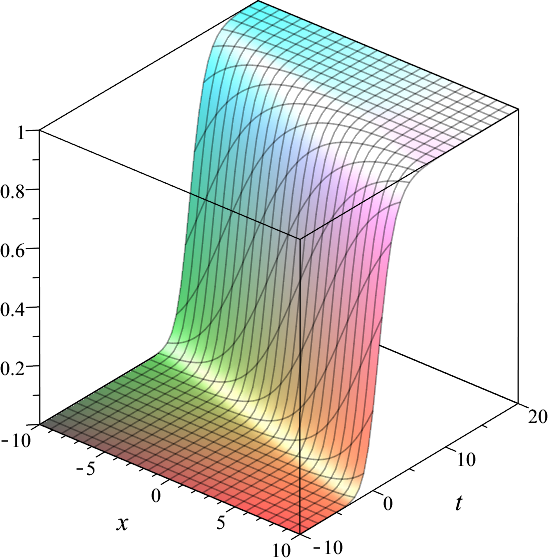
\includegraphics[width=.45\textwidth]{fig/(1+1)Fisher-tanh.png}
\caption{(1+1)维 Fisher方程的双曲正切解\label{fisher-tanh}}
\end{figure}
    
\end{example}

对于一些带参数的方程, 有时需要探索方程是否在某些参数条件下有解. 所以我们将在下一个例子中展示参数\cd{SP}的作用.

\begin{example}可以求解出相应的参数约束条件. 

对于(1+1)维 7阶色散方程\cite{duffy1996travelling}
\begin{equation}
    {{u}_{t}}+u\,{{u}_{x}}+p\,{{u}_{3x}}+q\,{{u}_{5x}}+r\,{{u}_{7x}}=0,
\end{equation}
设$\xi=kx+ct+\eta$. 若调用
\begin{verbatim}
nctm(eq,a,[k,c,eta]);
\end{verbatim}
则无解. 此时, 我们允许参数$r$被其它参数表示, 调用
\begin{verbatim}
nctm(eq,a,[k,c,eta],SP={r});
\end{verbatim}
可以确定$m=6$, 并得到6个解:
\begin{equation}
\renewcommand{\arraystretch}{1.4}
\begin{array}{rl}
r=0:& u=\pm \frac{2\,q\,\sqrt {13}\,c}{\sqrt {-p\,q}}-\frac{3\,{p}^{2}\,\left( 35\,{T}^{4}-70\,{T}^{2}+23\right) }{169\,q},k=-\frac{\sqrt {13}\,\sqrt {-p\,q}}{26\,q};\\
r=\frac{769 q^2}{2500 p}:& u=\frac{1538\,c\,q\,k}{25\,p}+\frac{2250\,{p}^{2}\,\left( 231\,{T}^{6}-693\,{T}^{4}+693\,{T}^{2}-151\right) }{591361\,q},k=\pm \frac{5\,\sqrt {1538}\,\sqrt {-p\,q}}{1538\,q};\\
r=\frac{2519 q^2}{10000 p}:& u=\frac{2159\,c\,q\,k}{25\,p}+\frac{500\,{p}^{2}\,\left( 2079\,{T}^{6}-8316\,{T}^{4}+10395\,{T}^{2}-2738\right) }{4661281\,q},k=\pm\frac{5\,\sqrt {2159}\,\sqrt {-p\,q}}{2159\,q}, \\
\end{array}
\end{equation}
其中 $T=\tanh\sbrace{kx+ct+\eta}$. 

因为\cd{PDEtools:-TWSolutions} 不支持对参数进行求解, 所以我们将此结果和 RATH 进行比较. 即使删去$r=0$时的两个解, 我们的解依然比 RATH\cite[p21]{liu2001master} 丰富, 因为 RATH 只给出了$r=\frac{769 q^2}{2500 p}$和$r=\frac{2519 q^2}{10000 p}$时的两个解.
\end{example}

虽然现有的双曲正切方法能够在只考虑第一类平衡点的情况下完成求解, 但是只要有阶数相同的最高项存在, 就不能排除另外两类平衡点存在的可能性. 但是, 基于$n$阶展开方法就能排除漏解的可能性, (4+1)维 Fokas方程就是一个典型的例子.

\begin{example}含全部三类平衡点

对于(4+1)维 Fokas方程\CITEdaFokas{}
\begin{equation}
    u_{tx}-\frac{1}{4}u_{xxxy}+\frac{1}{4}u_{xyyy}+3u_xu_y+3uu_{xy}-\frac{3}{2}u_{wz}=0 ,
\end{equation}
其阶数列表为$\mbrace{2m+2,m+4,m+4,2m+2,m+2}$. 
\begin{compactitem}[\textbullet]
\item 首先, 根据$2m+2=m+4$可以得到第一类平衡点$m=2$.
\item 然后, 考虑$m+4=m+4$, 根据最大性约束有$m+4>2m+2$, 可得$m<2$, 所以有第二类平衡点$m=1$.
\item 最后, 因为有两个$2m+2$, 所以需要考虑第三类平衡点. 我们取$\xi=kx+py+qz+rw+ct+\eta$, 代入后可得$n$阶展开的第一个非零项
\begin{equation}
    \Omega_0 = 24kpa_0^2m\sbrace{m+\frac{1}{2}}. 
\end{equation}
因为$\Omega_0=0$关于$m$没有正整数解, 所以需要$2m+2\le m+4$, 从而得到第三类平衡点的上界为$m=2$.
\end{compactitem}
   
最终, 我们确定$m=2$, 这既是第一类平衡点, 也是第三类平衡点. \cd{NTCM}给出了原方程的两个解
\begin{equation}
    \left\{ k=\pm \sqrt {{p}^{2}+{{a}_{2}}},{{a}_{0}}=-\frac{2\,{{a}_{2}}}{3}-\frac{c}{3\,p}+ \frac{q\,r}{2\,k\,p},{{a}_{1}}=0\right\} .
\end{equation}
\end{example}

在之前的例子中, 第三类平衡点并没有起到决定性的作用. 最后, 我们再通过一个只有第三类平衡点的例子来展示\cd{NTCM}中由$n$阶展开方法带来的优势.

\begin{example} 第三类平衡点的主导作用 

考虑
\begin{equation}
    u(u_t+u_{xxx})+pu_x u_{xx}=0.
\end{equation}
取$\xi=kx+ct+\eta$, 我们调用\cd{nctm(eq,a,[k,c,eta])}进行求解. 原方程的阶数列表为$\mbrace{2m+1,2m+3,2m+3}$, 只存在\BPthree{}. 由
\begin{equation}
    \Omega_0=-{{{a}_{0}}}^{2}\,m\,\left( m\,p+m+2\right) \,\left( m+1\right) \,{k}^{3}
\end{equation}
得到$m=0$. 从而原方程没有非平凡的解. 但是, $m$还有一个可能的零点$m=\frac{-2}{p+1}$. 从而, 当$p$的取值合适时, 原方程可能有任意次数的解. 事实上, \cd{NTCM}能够发现此类情况并输出警告. 

取$p=-3$可以得到$m=1$, 原方程有解 
\begin{equation}
    \left\{ c=-4\,{k}^{3},{{a}_{0}}=0, a_1=a_1\right\} .
\end{equation}

此外, 我们总结出: 当$n\ge 1$时, 若$p=-\frac{n+1}{n}$, 则$m=2n$, 原方程有解 
\begin{equation}
    u=(-1)^n a_{2n} \sbrace{\tanh^2(kx+4nk^3t+\eta)-1}^n. 
\end{equation}


事实上, \cd{PDEtools:-TWSolutions}在遇到这种情况时, 会取$m=3$进行尝试. 所以, NCTM 能够求得\cd{PDEtools:-TWSolutions}无法求得的解. 
\end{example}


\begin{example} 
考虑方程 \cite{EMM}
\begin{equation}
    {{u}_{t}}+{{u}_{x}}+\alpha\,{{u}_{xxx}}+\beta\,u\,{{u}_{x}}+\gamma\,u\,{{u}_{xxx}}+\delta\,{{u}_{x}}\,{{u}_{xx}}=0,
\end{equation}
这是一个从弹性介质的微观结构中导出的非线性演化方程. 取$\xi=kx+ct+\eta$, 调用\cd{nctm(eq,a,[k,c,eta])}进行求解, 可得其阶数列表为$[m+1,m+1,2m+1,2m+3,2m+3]$. 由
\begin{equation}
    \Omega_0=-{{{a}_{0}}}^{2}\,{k}^{3}\,m\,\left( m+1\right) \,\left( m\,\delta+\gamma\,m+2\,\gamma\right)
\end{equation}
可得 $m=0$, 原方程没有非平凡的解. 当$m=\frac{-2 \gamma}{\gamma+\delta}$为正整数时, 就存在其它可能的平衡点.

这和上一个例子一样, 也是一个可以任意阶平衡的方程, 解的形式为
\begin{equation}
    u=a_0 + a_1 \tanh(\xi) + \cdots + a_m \tanh^m(\xi), ~ \xi = kx+ct+\eta . 
\end{equation}

当$\gamma=-1,\delta=3$时, $m=1$, 原方程有两个解 
\begin{equation}
    \bbrace{a_0=\alpha,k=\pm\frac{\sqrt{\beta}}{2},c=-k\frac{\alpha \beta+1}{2},a_1=a_1}.
\end{equation}

此外, 我们总结出: 当$n\ge 1$时, 若$\gamma=-n,\delta=n+1$, 则$m=2n$, 原方程有解 
\begin{equation}
u=(-1)^n a_{2n} \sbrace{\tanh^2\sbrace{\frac{\pm\sqrt{-\beta}}{2n}x-\frac{\pm\sqrt{-\beta}(\alpha\beta+n)}{2n^2}t+\eta}-1}^n+\frac{\alpha}{n} .
\end{equation}
\end{example}

\section{$n$阶展开方法在\Painleve{}展开法中的应用}\label{ch4sec6}
在\Painleve{}展开法中, 假设 
\begin{equation}
    u=\sum_{k=1}^{m}\frac{u_k}{f^{m-k+1}}. \label{TPE-pkg}
\end{equation}
我们可以将其看作是关于$1/f$的多项式
\begin{equation}
    u=F\sbrace{\frac{1}{f},m,\mu\up{n}}.
\end{equation}
在应用$n$阶展开方法时, 因为 
\begin{equation}
    \DIF{x}{\frac{1}{f}}=-\frac{f_x}{f^2}=F\sbrace{\frac{1}{f},2,\mbrace{-f_x,0,0}},
\end{equation}
也能根据\refeqn{NEM-diff}完成求导操作. 

在将$u$及其导数转化为关于$1/f$的$n$阶展开多项式之后, 利用\cd{NEPoly}对象的乘法操作, 可以将原方程的各个加法项也转化为\cd{NEPoly}对象. 然后, 我们就可以利用\cd{nem}来分析$m$的上界. 之后, 我们就可以将\refeqn{TPE-pkg}代入原方程, 利用\refalg{rpsolve}实现待定系数的求解. 对于\refalg{rpsolve}的求解结果, 我们会删去全零的解. 最终, 我们将返回输入方程的 TPE. 

基于上述方法, 我们实现了 PExpand 软件包. PExpand 的核心接口为
\begin{verbatim}
ftr:=panalyze(eq,u,f,{nExpand,selelct_solution});
\end{verbatim}
其中
\begin{compactitem}[\textbullet]
\item \cd{eq}表示输入的方程, \cd{u}表示方程中的未知函数, \cd{f}表示变换后的未知函数, 要求\cd{u}和\cd{f}拥有相同的自变量.
\item 可选参数\cd{nExpand}表示$n$阶展开的阶数, 默认值为2.
\item 可选参数\cd{select\_solution}的作用和\cd{twsolve}中的同名参数一样, 用于允许用户通过交互的方式选择解. 如果不指定该参数, 函数将默认返回第一个解. 
\item 返回值\cd{ftr}表示形如\refeqn{TPE-pkg}的TPE. 
\end{compactitem}

下面以一个典型的例子来展示 NEM 在\Painleve{}展开法中的应用.

\begin{example}
考虑方程
\begin{equation}
    u(u_t+u_{xxx})-3u_x u_{xx}=0. \label{pseq}
\end{equation}
其阶数列表为$\mbrace{2m+1,2m+3,2m+3}$, 只有\BPthree{}. 由
\begin{equation}
    \Omega_0=2m(m^2-1)u_0^2f_x^3
\end{equation}
可得$m=1$. 将$u=\mu/f$代入原方程后, 关于$1/f$的最高项系数为
\begin{equation}
    3\,\mu\,{{f}_{x}}\,\left( \mu\,{{f}_{xx}}-2\,{{\mu}_{x}}\,{{f}_{x}}\right) .
\end{equation}
可以解得 
\begin{equation}
    \mu=F(t)\sqrt{f_x}.
\end{equation}
\end{example}
我们取$\mu=\sqrt{f_x}$, 即$u=\sqrt{f_x}/f$代入\refeqnn{pseq}, 可以得到
\begin{equation}
\begin{aligned}
& 2\,{{f}_{tx}}\,{{{f}_{x}}}^{2}\,f+2\,{{f}_{xxxx}}\,{{{f}_{x}}}^{2}\,f-6\,{{f}_{xx}}\,{{f}_{xxx}}\,{{f}_{x}}\,f+3\,{{{f}_{xx}}}^{3}\,f \\
-&4\,{{{f}_{x}}}^{3}\,{{f}_{t}}-4\,{{f}_{xxx}}\,{{{f}_{x}}}^{3}+6\,{{{f}_{xx}}}^{2}\,{{{f}_{x}}}^{2}=0.
\end{aligned} \label{pseq-f}
\end{equation}
随后, 我们就能基于\refeqnn{pseq-f}进行各种类型的解的求解.

事实上, 本文所实现的 PExpand 软件包能够自动导出变换$u=F(t)\sqrt{f_x}/f$, 但是我们不能以这个变换为基础进行后续的求解.  因此, 本文实现的 TwSolver 和 NS1L 都不能直接求解\refeqnn{raeq}. 但是, 这两个软件包都提供了自定义变换进行求解的功能.

在TwSolver中, 调用
\begin{verbatim}
twsolve(
    eq,{1},PL=[k,c],
    _utr=(f->sqrt(diff(f,x))/f)
);
\end{verbatim}
就能够指定变换进行求解. 该方程在简单Hirota方法下只有1-孤子解
\begin{equation}
    f=1+\exp\sbrace{k\sbrace{x+\frac{k^2}{2}t}+c}.
\end{equation}
在NS1L中, 也可以利用参数\cd{\_utr=(f->sqrt(diff(f,x))/f)}指定变换进行求解. 不过, 该方程没有lump解.

\begin{example} 
考虑方程 \cite{EMM}
\begin{equation}
    {{u}_{t}}+{{u}_{x}}+\alpha\,{{u}_{xxx}}+\beta\,u\,{{u}_{x}}+\gamma\,u\,{{u}_{xxx}}+\delta\,{{u}_{x}}\,{{u}_{xx}}=0,
\end{equation}
其阶数列表为$[m+1,m+1,2m+1,2m+3,2m+3]$, 只有第三类平衡点. 对该方程进行1阶展开, 即取$u=\mu_0/f^m+\OO(1/f^{m-1})$代入原方程, 可以得到
\begin{equation}
    -\mu_0^2f_x^3m(m+1)(\gamma m+\delta m+2\gamma)\frac{1}{f^{2m+3}}+\OO\sbrace{\frac{1}{f^{2m+2}}}=0. 
\end{equation}
当$\gamma=-1,\delta=3$时, $m=1$, PExpand 可以解得 
\begin{equation}
    u=\frac{\sqrt{f_x}}{f}\sbrace{\alpha\int\!{\sqrt{f_x}{\,\rm d}x}+F(t)}.
\end{equation}
而其它软件只能得到$m=0$, 从而无法继续求解. 
\end{example}

\section{小结}\label{ch4sec7}

在本章中, 我们提出了$n$阶展开方法来完善齐次平衡原则, 并将其应用于微分方程和差分方程的若干求解方法中. 我们针对$n$阶展开方法开发了 NEM 软件包, 并在此基础上开发了求解非线性差分方程多项式解的软件包NLREPS. 同时, 我们还将$n$阶展开方法应用于微分方程的求解. 我们开发了基于双曲正切方法的 NCTM 和实现\Painleve{}展开法的 PExpand. 

实验和例子表明, $n$阶展开方法确实完善了齐次平衡原则, 能更加全面的分析平衡的情况, 在求解时获得更多的解. 此外, 对于大部分的方程, 展开阶数为2已经能够完成求解. 

本章的成果已被华东师范大学学报(自然科学版)接受.
